% Created by tikzDevice version 0.12.3 on 2019-09-27 19:56:29
% !TEX encoding = UTF-8 Unicode
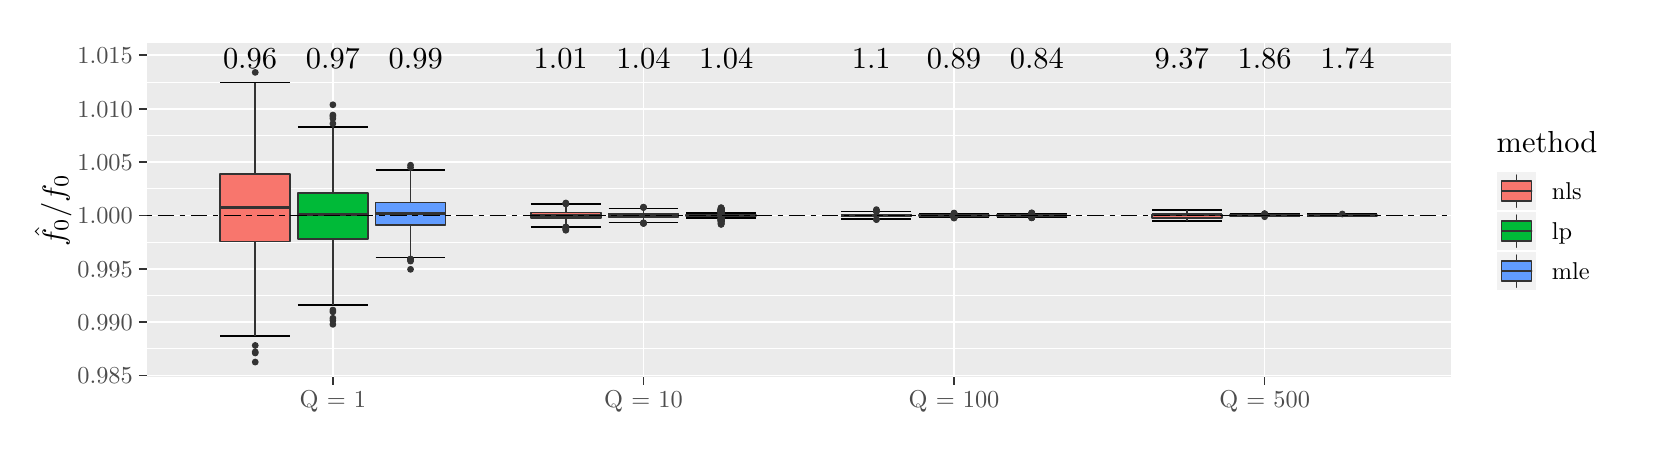
\begin{tikzpicture}[x=1pt,y=1pt]
\definecolor{fillColor}{RGB}{255,255,255}
\path[use as bounding box,fill=fillColor,fill opacity=0.00] (0,0) rectangle (578.16,144.54);
\begin{scope}
\path[clip] (  0.00,  0.00) rectangle (578.16,144.54);
\definecolor{drawColor}{RGB}{255,255,255}
\definecolor{fillColor}{RGB}{255,255,255}

\path[draw=drawColor,line width= 0.6pt,line join=round,line cap=round,fill=fillColor] (  0.00,  0.00) rectangle (578.16,144.54);
\end{scope}
\begin{scope}
\path[clip] ( 42.95, 18.22) rectangle (514.31,139.04);
\definecolor{fillColor}{gray}{0.92}

\path[fill=fillColor] ( 42.95, 18.22) rectangle (514.31,139.04);
\definecolor{drawColor}{RGB}{255,255,255}

\path[draw=drawColor,line width= 0.3pt,line join=round] ( 42.95, 28.49) --
	(514.31, 28.49);

\path[draw=drawColor,line width= 0.3pt,line join=round] ( 42.95, 47.77) --
	(514.31, 47.77);

\path[draw=drawColor,line width= 0.3pt,line join=round] ( 42.95, 67.06) --
	(514.31, 67.06);

\path[draw=drawColor,line width= 0.3pt,line join=round] ( 42.95, 86.34) --
	(514.31, 86.34);

\path[draw=drawColor,line width= 0.3pt,line join=round] ( 42.95,105.63) --
	(514.31,105.63);

\path[draw=drawColor,line width= 0.3pt,line join=round] ( 42.95,124.91) --
	(514.31,124.91);

\path[draw=drawColor,line width= 0.6pt,line join=round] ( 42.95, 18.84) --
	(514.31, 18.84);

\path[draw=drawColor,line width= 0.6pt,line join=round] ( 42.95, 38.13) --
	(514.31, 38.13);

\path[draw=drawColor,line width= 0.6pt,line join=round] ( 42.95, 57.41) --
	(514.31, 57.41);

\path[draw=drawColor,line width= 0.6pt,line join=round] ( 42.95, 76.70) --
	(514.31, 76.70);

\path[draw=drawColor,line width= 0.6pt,line join=round] ( 42.95, 95.99) --
	(514.31, 95.99);

\path[draw=drawColor,line width= 0.6pt,line join=round] ( 42.95,115.27) --
	(514.31,115.27);

\path[draw=drawColor,line width= 0.6pt,line join=round] ( 42.95,134.56) --
	(514.31,134.56);

\path[draw=drawColor,line width= 0.6pt,line join=round] (110.29, 18.22) --
	(110.29,139.04);

\path[draw=drawColor,line width= 0.6pt,line join=round] (222.52, 18.22) --
	(222.52,139.04);

\path[draw=drawColor,line width= 0.6pt,line join=round] (334.74, 18.22) --
	(334.74,139.04);

\path[draw=drawColor,line width= 0.6pt,line join=round] (446.97, 18.22) --
	(446.97,139.04);
\definecolor{drawColor}{RGB}{0,0,0}

\path[draw=drawColor,line width= 0.6pt,line join=round] ( 69.61,124.67) --
	( 94.86,124.67);

\path[draw=drawColor,line width= 0.6pt,line join=round] ( 82.23,124.67) --
	( 82.23, 33.03);

\path[draw=drawColor,line width= 0.6pt,line join=round] ( 69.61, 33.03) --
	( 94.86, 33.03);

\path[draw=drawColor,line width= 0.6pt,line join=round] ( 97.66,108.56) --
	(122.92,108.56);

\path[draw=drawColor,line width= 0.6pt,line join=round] (110.29,108.56) --
	(110.29, 44.37);

\path[draw=drawColor,line width= 0.6pt,line join=round] ( 97.66, 44.37) --
	(122.92, 44.37);

\path[draw=drawColor,line width= 0.6pt,line join=round] (125.72, 93.16) --
	(150.97, 93.16);

\path[draw=drawColor,line width= 0.6pt,line join=round] (138.35, 93.16) --
	(138.35, 61.46);

\path[draw=drawColor,line width= 0.6pt,line join=round] (125.72, 61.46) --
	(150.97, 61.46);

\path[draw=drawColor,line width= 0.6pt,line join=round] (181.83, 80.83) --
	(207.09, 80.83);

\path[draw=drawColor,line width= 0.6pt,line join=round] (194.46, 80.83) --
	(194.46, 72.57);

\path[draw=drawColor,line width= 0.6pt,line join=round] (181.83, 72.57) --
	(207.09, 72.57);

\path[draw=drawColor,line width= 0.6pt,line join=round] (209.89, 79.17) --
	(235.14, 79.17);

\path[draw=drawColor,line width= 0.6pt,line join=round] (222.52, 79.17) --
	(222.52, 74.08);

\path[draw=drawColor,line width= 0.6pt,line join=round] (209.89, 74.08) --
	(235.14, 74.08);

\path[draw=drawColor,line width= 0.6pt,line join=round] (237.95, 77.51) --
	(263.20, 77.51);

\path[draw=drawColor,line width= 0.6pt,line join=round] (250.57, 77.51) --
	(250.57, 75.79);

\path[draw=drawColor,line width= 0.6pt,line join=round] (237.95, 75.79) --
	(263.20, 75.79);

\path[draw=drawColor,line width= 0.6pt,line join=round] (294.06, 78.07) --
	(319.31, 78.07);

\path[draw=drawColor,line width= 0.6pt,line join=round] (306.69, 78.07) --
	(306.69, 75.32);

\path[draw=drawColor,line width= 0.6pt,line join=round] (294.06, 75.32) --
	(319.31, 75.32);

\path[draw=drawColor,line width= 0.6pt,line join=round] (322.12, 77.36) --
	(347.37, 77.36);

\path[draw=drawColor,line width= 0.6pt,line join=round] (334.74, 77.36) --
	(334.74, 76.00);

\path[draw=drawColor,line width= 0.6pt,line join=round] (322.12, 76.00) --
	(347.37, 76.00);

\path[draw=drawColor,line width= 0.6pt,line join=round] (350.18, 77.37) --
	(375.43, 77.37);

\path[draw=drawColor,line width= 0.6pt,line join=round] (362.80, 77.37) --
	(362.80, 76.00);

\path[draw=drawColor,line width= 0.6pt,line join=round] (350.18, 76.00) --
	(375.43, 76.00);

\path[draw=drawColor,line width= 0.6pt,line join=round] (406.29, 78.73) --
	(431.54, 78.73);

\path[draw=drawColor,line width= 0.6pt,line join=round] (418.91, 78.73) --
	(418.91, 74.74);

\path[draw=drawColor,line width= 0.6pt,line join=round] (406.29, 74.74) --
	(431.54, 74.74);

\path[draw=drawColor,line width= 0.6pt,line join=round] (434.35, 77.15) --
	(459.60, 77.15);

\path[draw=drawColor,line width= 0.6pt,line join=round] (446.97, 77.15) --
	(446.97, 76.26);

\path[draw=drawColor,line width= 0.6pt,line join=round] (434.35, 76.26) --
	(459.60, 76.26);

\path[draw=drawColor,line width= 0.6pt,line join=round] (462.40, 77.16) --
	(487.65, 77.16);

\path[draw=drawColor,line width= 0.6pt,line join=round] (475.03, 77.16) --
	(475.03, 76.27);

\path[draw=drawColor,line width= 0.6pt,line join=round] (462.40, 76.27) --
	(487.65, 76.27);
\definecolor{drawColor}{gray}{0.20}
\definecolor{fillColor}{gray}{0.20}

\path[draw=drawColor,line width= 0.4pt,line join=round,line cap=round,fill=fillColor] ( 82.23, 27.38) circle (  1.02);

\path[draw=drawColor,line width= 0.4pt,line join=round,line cap=round,fill=fillColor] ( 82.23, 23.71) circle (  1.02);

\path[draw=drawColor,line width= 0.4pt,line join=round,line cap=round,fill=fillColor] ( 82.23,128.38) circle (  1.02);

\path[draw=drawColor,line width= 0.4pt,line join=round,line cap=round,fill=fillColor] ( 82.23, 29.71) circle (  1.02);

\path[draw=drawColor,line width= 0.4pt,line join=round,line cap=round,fill=fillColor] ( 82.23, 26.99) circle (  1.02);

\path[draw=drawColor,line width= 0.6pt,line join=round] ( 82.23, 91.70) -- ( 82.23,124.67);

\path[draw=drawColor,line width= 0.6pt,line join=round] ( 82.23, 67.31) -- ( 82.23, 33.03);
\definecolor{fillColor}{RGB}{248,118,109}

\path[draw=drawColor,line width= 0.6pt,line join=round,line cap=round,fill=fillColor] ( 69.61, 91.70) --
	( 69.61, 67.31) --
	( 94.86, 67.31) --
	( 94.86, 91.70) --
	( 69.61, 91.70) --
	cycle;

\path[draw=drawColor,line width= 1.1pt,line join=round] ( 69.61, 79.60) -- ( 94.86, 79.60);
\definecolor{fillColor}{gray}{0.20}

\path[draw=drawColor,line width= 0.4pt,line join=round,line cap=round,fill=fillColor] (110.29,112.98) circle (  1.02);

\path[draw=drawColor,line width= 0.4pt,line join=round,line cap=round,fill=fillColor] (110.29, 38.76) circle (  1.02);

\path[draw=drawColor,line width= 0.4pt,line join=round,line cap=round,fill=fillColor] (110.29,112.53) circle (  1.02);

\path[draw=drawColor,line width= 0.4pt,line join=round,line cap=round,fill=fillColor] (110.29,109.87) circle (  1.02);

\path[draw=drawColor,line width= 0.4pt,line join=round,line cap=round,fill=fillColor] (110.29,116.68) circle (  1.02);

\path[draw=drawColor,line width= 0.4pt,line join=round,line cap=round,fill=fillColor] (110.29, 37.34) circle (  1.02);

\path[draw=drawColor,line width= 0.4pt,line join=round,line cap=round,fill=fillColor] (110.29, 42.51) circle (  1.02);

\path[draw=drawColor,line width= 0.4pt,line join=round,line cap=round,fill=fillColor] (110.29,111.73) circle (  1.02);

\path[draw=drawColor,line width= 0.4pt,line join=round,line cap=round,fill=fillColor] (110.29, 39.55) circle (  1.02);

\path[draw=drawColor,line width= 0.4pt,line join=round,line cap=round,fill=fillColor] (110.29, 41.85) circle (  1.02);

\path[draw=drawColor,line width= 0.6pt,line join=round] (110.29, 84.71) -- (110.29,108.56);

\path[draw=drawColor,line width= 0.6pt,line join=round] (110.29, 68.07) -- (110.29, 44.37);
\definecolor{fillColor}{RGB}{0,186,56}

\path[draw=drawColor,line width= 0.6pt,line join=round,line cap=round,fill=fillColor] ( 97.66, 84.71) --
	( 97.66, 68.07) --
	(122.92, 68.07) --
	(122.92, 84.71) --
	( 97.66, 84.71) --
	cycle;

\path[draw=drawColor,line width= 1.1pt,line join=round] ( 97.66, 77.11) -- (122.92, 77.11);
\definecolor{fillColor}{gray}{0.20}

\path[draw=drawColor,line width= 0.4pt,line join=round,line cap=round,fill=fillColor] (138.35, 60.83) circle (  1.02);

\path[draw=drawColor,line width= 0.4pt,line join=round,line cap=round,fill=fillColor] (138.35, 60.81) circle (  1.02);

\path[draw=drawColor,line width= 0.4pt,line join=round,line cap=round,fill=fillColor] (138.35, 57.21) circle (  1.02);

\path[draw=drawColor,line width= 0.4pt,line join=round,line cap=round,fill=fillColor] (138.35, 60.94) circle (  1.02);

\path[draw=drawColor,line width= 0.4pt,line join=round,line cap=round,fill=fillColor] (138.35, 93.99) circle (  1.02);

\path[draw=drawColor,line width= 0.4pt,line join=round,line cap=round,fill=fillColor] (138.35, 94.85) circle (  1.02);

\path[draw=drawColor,line width= 0.4pt,line join=round,line cap=round,fill=fillColor] (138.35, 60.19) circle (  1.02);

\path[draw=drawColor,line width= 0.6pt,line join=round] (138.35, 81.33) -- (138.35, 93.16);

\path[draw=drawColor,line width= 0.6pt,line join=round] (138.35, 73.35) -- (138.35, 61.46);
\definecolor{fillColor}{RGB}{97,156,255}

\path[draw=drawColor,line width= 0.6pt,line join=round,line cap=round,fill=fillColor] (125.72, 81.33) --
	(125.72, 73.35) --
	(150.97, 73.35) --
	(150.97, 81.33) --
	(125.72, 81.33) --
	cycle;

\path[draw=drawColor,line width= 1.1pt,line join=round] (125.72, 77.45) -- (150.97, 77.45);
\definecolor{fillColor}{gray}{0.20}

\path[draw=drawColor,line width= 0.4pt,line join=round,line cap=round,fill=fillColor] (194.46, 71.34) circle (  1.02);

\path[draw=drawColor,line width= 0.4pt,line join=round,line cap=round,fill=fillColor] (194.46, 72.39) circle (  1.02);

\path[draw=drawColor,line width= 0.4pt,line join=round,line cap=round,fill=fillColor] (194.46, 72.40) circle (  1.02);

\path[draw=drawColor,line width= 0.4pt,line join=round,line cap=round,fill=fillColor] (194.46, 71.56) circle (  1.02);

\path[draw=drawColor,line width= 0.4pt,line join=round,line cap=round,fill=fillColor] (194.46, 71.97) circle (  1.02);

\path[draw=drawColor,line width= 0.4pt,line join=round,line cap=round,fill=fillColor] (194.46, 72.45) circle (  1.02);

\path[draw=drawColor,line width= 0.4pt,line join=round,line cap=round,fill=fillColor] (194.46, 80.94) circle (  1.02);

\path[draw=drawColor,line width= 0.4pt,line join=round,line cap=round,fill=fillColor] (194.46, 81.19) circle (  1.02);

\path[draw=drawColor,line width= 0.4pt,line join=round,line cap=round,fill=fillColor] (194.46, 80.86) circle (  1.02);

\path[draw=drawColor,line width= 0.4pt,line join=round,line cap=round,fill=fillColor] (194.46, 72.52) circle (  1.02);

\path[draw=drawColor,line width= 0.4pt,line join=round,line cap=round,fill=fillColor] (194.46, 72.35) circle (  1.02);

\path[draw=drawColor,line width= 0.6pt,line join=round] (194.46, 77.73) -- (194.46, 80.83);

\path[draw=drawColor,line width= 0.6pt,line join=round] (194.46, 75.65) -- (194.46, 72.57);
\definecolor{fillColor}{RGB}{248,118,109}

\path[draw=drawColor,line width= 0.6pt,line join=round,line cap=round,fill=fillColor] (181.83, 77.73) --
	(181.83, 75.65) --
	(207.09, 75.65) --
	(207.09, 77.73) --
	(181.83, 77.73) --
	cycle;

\path[draw=drawColor,line width= 1.1pt,line join=round] (181.83, 76.53) -- (207.09, 76.53);
\definecolor{fillColor}{gray}{0.20}

\path[draw=drawColor,line width= 0.4pt,line join=round,line cap=round,fill=fillColor] (222.52, 73.80) circle (  1.02);

\path[draw=drawColor,line width= 0.4pt,line join=round,line cap=round,fill=fillColor] (222.52, 74.02) circle (  1.02);

\path[draw=drawColor,line width= 0.4pt,line join=round,line cap=round,fill=fillColor] (222.52, 79.57) circle (  1.02);

\path[draw=drawColor,line width= 0.4pt,line join=round,line cap=round,fill=fillColor] (222.52, 79.63) circle (  1.02);

\path[draw=drawColor,line width= 0.4pt,line join=round,line cap=round,fill=fillColor] (222.52, 73.91) circle (  1.02);

\path[draw=drawColor,line width= 0.4pt,line join=round,line cap=round,fill=fillColor] (222.52, 73.82) circle (  1.02);

\path[draw=drawColor,line width= 0.4pt,line join=round,line cap=round,fill=fillColor] (222.52, 79.63) circle (  1.02);

\path[draw=drawColor,line width= 0.6pt,line join=round] (222.52, 77.34) -- (222.52, 79.17);

\path[draw=drawColor,line width= 0.6pt,line join=round] (222.52, 76.02) -- (222.52, 74.08);
\definecolor{fillColor}{RGB}{0,186,56}

\path[draw=drawColor,line width= 0.6pt,line join=round,line cap=round,fill=fillColor] (209.89, 77.34) --
	(209.89, 76.02) --
	(235.14, 76.02) --
	(235.14, 77.34) --
	(209.89, 77.34) --
	cycle;

\path[draw=drawColor,line width= 1.1pt,line join=round] (209.89, 76.68) -- (235.14, 76.68);
\definecolor{fillColor}{gray}{0.20}

\path[draw=drawColor,line width= 0.4pt,line join=round,line cap=round,fill=fillColor] (250.57, 77.89) circle (  1.02);

\path[draw=drawColor,line width= 0.4pt,line join=round,line cap=round,fill=fillColor] (250.57, 75.45) circle (  1.02);

\path[draw=drawColor,line width= 0.4pt,line join=round,line cap=round,fill=fillColor] (250.57, 77.80) circle (  1.02);

\path[draw=drawColor,line width= 0.4pt,line join=round,line cap=round,fill=fillColor] (250.57, 78.38) circle (  1.02);

\path[draw=drawColor,line width= 0.4pt,line join=round,line cap=round,fill=fillColor] (250.57, 78.67) circle (  1.02);

\path[draw=drawColor,line width= 0.4pt,line join=round,line cap=round,fill=fillColor] (250.57, 77.74) circle (  1.02);

\path[draw=drawColor,line width= 0.4pt,line join=round,line cap=round,fill=fillColor] (250.57, 78.49) circle (  1.02);

\path[draw=drawColor,line width= 0.4pt,line join=round,line cap=round,fill=fillColor] (250.57, 75.35) circle (  1.02);

\path[draw=drawColor,line width= 0.4pt,line join=round,line cap=round,fill=fillColor] (250.57, 78.21) circle (  1.02);

\path[draw=drawColor,line width= 0.4pt,line join=round,line cap=round,fill=fillColor] (250.57, 77.53) circle (  1.02);

\path[draw=drawColor,line width= 0.4pt,line join=round,line cap=round,fill=fillColor] (250.57, 73.79) circle (  1.02);

\path[draw=drawColor,line width= 0.4pt,line join=round,line cap=round,fill=fillColor] (250.57, 78.25) circle (  1.02);

\path[draw=drawColor,line width= 0.4pt,line join=round,line cap=round,fill=fillColor] (250.57, 77.92) circle (  1.02);

\path[draw=drawColor,line width= 0.4pt,line join=round,line cap=round,fill=fillColor] (250.57, 78.99) circle (  1.02);

\path[draw=drawColor,line width= 0.4pt,line join=round,line cap=round,fill=fillColor] (250.57, 78.54) circle (  1.02);

\path[draw=drawColor,line width= 0.4pt,line join=round,line cap=round,fill=fillColor] (250.57, 73.90) circle (  1.02);

\path[draw=drawColor,line width= 0.4pt,line join=round,line cap=round,fill=fillColor] (250.57, 78.54) circle (  1.02);

\path[draw=drawColor,line width= 0.4pt,line join=round,line cap=round,fill=fillColor] (250.57, 78.31) circle (  1.02);

\path[draw=drawColor,line width= 0.4pt,line join=round,line cap=round,fill=fillColor] (250.57, 78.07) circle (  1.02);

\path[draw=drawColor,line width= 0.4pt,line join=round,line cap=round,fill=fillColor] (250.57, 78.13) circle (  1.02);

\path[draw=drawColor,line width= 0.4pt,line join=round,line cap=round,fill=fillColor] (250.57, 78.41) circle (  1.02);

\path[draw=drawColor,line width= 0.4pt,line join=round,line cap=round,fill=fillColor] (250.57, 75.69) circle (  1.02);

\path[draw=drawColor,line width= 0.4pt,line join=round,line cap=round,fill=fillColor] (250.57, 74.87) circle (  1.02);

\path[draw=drawColor,line width= 0.4pt,line join=round,line cap=round,fill=fillColor] (250.57, 78.71) circle (  1.02);

\path[draw=drawColor,line width= 0.4pt,line join=round,line cap=round,fill=fillColor] (250.57, 74.37) circle (  1.02);

\path[draw=drawColor,line width= 0.4pt,line join=round,line cap=round,fill=fillColor] (250.57, 77.56) circle (  1.02);

\path[draw=drawColor,line width= 0.4pt,line join=round,line cap=round,fill=fillColor] (250.57, 77.61) circle (  1.02);

\path[draw=drawColor,line width= 0.4pt,line join=round,line cap=round,fill=fillColor] (250.57, 78.44) circle (  1.02);

\path[draw=drawColor,line width= 0.4pt,line join=round,line cap=round,fill=fillColor] (250.57, 78.83) circle (  1.02);

\path[draw=drawColor,line width= 0.4pt,line join=round,line cap=round,fill=fillColor] (250.57, 75.38) circle (  1.02);

\path[draw=drawColor,line width= 0.4pt,line join=round,line cap=round,fill=fillColor] (250.57, 77.91) circle (  1.02);

\path[draw=drawColor,line width= 0.4pt,line join=round,line cap=round,fill=fillColor] (250.57, 78.06) circle (  1.02);

\path[draw=drawColor,line width= 0.4pt,line join=round,line cap=round,fill=fillColor] (250.57, 74.71) circle (  1.02);

\path[draw=drawColor,line width= 0.4pt,line join=round,line cap=round,fill=fillColor] (250.57, 78.86) circle (  1.02);

\path[draw=drawColor,line width= 0.4pt,line join=round,line cap=round,fill=fillColor] (250.57, 79.32) circle (  1.02);

\path[draw=drawColor,line width= 0.4pt,line join=round,line cap=round,fill=fillColor] (250.57, 79.41) circle (  1.02);

\path[draw=drawColor,line width= 0.4pt,line join=round,line cap=round,fill=fillColor] (250.57, 75.15) circle (  1.02);

\path[draw=drawColor,line width= 0.4pt,line join=round,line cap=round,fill=fillColor] (250.57, 77.84) circle (  1.02);

\path[draw=drawColor,line width= 0.4pt,line join=round,line cap=round,fill=fillColor] (250.57, 78.81) circle (  1.02);

\path[draw=drawColor,line width= 0.4pt,line join=round,line cap=round,fill=fillColor] (250.57, 75.69) circle (  1.02);

\path[draw=drawColor,line width= 0.4pt,line join=round,line cap=round,fill=fillColor] (250.57, 74.73) circle (  1.02);

\path[draw=drawColor,line width= 0.4pt,line join=round,line cap=round,fill=fillColor] (250.57, 77.56) circle (  1.02);

\path[draw=drawColor,line width= 0.4pt,line join=round,line cap=round,fill=fillColor] (250.57, 78.14) circle (  1.02);

\path[draw=drawColor,line width= 0.4pt,line join=round,line cap=round,fill=fillColor] (250.57, 79.19) circle (  1.02);

\path[draw=drawColor,line width= 0.4pt,line join=round,line cap=round,fill=fillColor] (250.57, 77.82) circle (  1.02);

\path[draw=drawColor,line width= 0.4pt,line join=round,line cap=round,fill=fillColor] (250.57, 74.92) circle (  1.02);

\path[draw=drawColor,line width= 0.4pt,line join=round,line cap=round,fill=fillColor] (250.57, 77.65) circle (  1.02);

\path[draw=drawColor,line width= 0.4pt,line join=round,line cap=round,fill=fillColor] (250.57, 75.70) circle (  1.02);

\path[draw=drawColor,line width= 0.4pt,line join=round,line cap=round,fill=fillColor] (250.57, 78.04) circle (  1.02);

\path[draw=drawColor,line width= 0.4pt,line join=round,line cap=round,fill=fillColor] (250.57, 77.94) circle (  1.02);

\path[draw=drawColor,line width= 0.4pt,line join=round,line cap=round,fill=fillColor] (250.57, 75.51) circle (  1.02);

\path[draw=drawColor,line width= 0.4pt,line join=round,line cap=round,fill=fillColor] (250.57, 78.28) circle (  1.02);

\path[draw=drawColor,line width= 0.4pt,line join=round,line cap=round,fill=fillColor] (250.57, 75.06) circle (  1.02);

\path[draw=drawColor,line width= 0.4pt,line join=round,line cap=round,fill=fillColor] (250.57, 77.72) circle (  1.02);

\path[draw=drawColor,line width= 0.4pt,line join=round,line cap=round,fill=fillColor] (250.57, 75.71) circle (  1.02);

\path[draw=drawColor,line width= 0.4pt,line join=round,line cap=round,fill=fillColor] (250.57, 77.88) circle (  1.02);

\path[draw=drawColor,line width= 0.4pt,line join=round,line cap=round,fill=fillColor] (250.57, 78.89) circle (  1.02);

\path[draw=drawColor,line width= 0.4pt,line join=round,line cap=round,fill=fillColor] (250.57, 78.56) circle (  1.02);

\path[draw=drawColor,line width= 0.4pt,line join=round,line cap=round,fill=fillColor] (250.57, 79.10) circle (  1.02);

\path[draw=drawColor,line width= 0.4pt,line join=round,line cap=round,fill=fillColor] (250.57, 74.80) circle (  1.02);

\path[draw=drawColor,line width= 0.4pt,line join=round,line cap=round,fill=fillColor] (250.57, 73.50) circle (  1.02);

\path[draw=drawColor,line width= 0.4pt,line join=round,line cap=round,fill=fillColor] (250.57, 78.17) circle (  1.02);

\path[draw=drawColor,line width= 0.4pt,line join=round,line cap=round,fill=fillColor] (250.57, 77.86) circle (  1.02);

\path[draw=drawColor,line width= 0.4pt,line join=round,line cap=round,fill=fillColor] (250.57, 78.34) circle (  1.02);

\path[draw=drawColor,line width= 0.4pt,line join=round,line cap=round,fill=fillColor] (250.57, 78.66) circle (  1.02);

\path[draw=drawColor,line width= 0.4pt,line join=round,line cap=round,fill=fillColor] (250.57, 78.01) circle (  1.02);

\path[draw=drawColor,line width= 0.4pt,line join=round,line cap=round,fill=fillColor] (250.57, 77.72) circle (  1.02);

\path[draw=drawColor,line width= 0.4pt,line join=round,line cap=round,fill=fillColor] (250.57, 78.07) circle (  1.02);

\path[draw=drawColor,line width= 0.4pt,line join=round,line cap=round,fill=fillColor] (250.57, 74.77) circle (  1.02);

\path[draw=drawColor,line width= 0.4pt,line join=round,line cap=round,fill=fillColor] (250.57, 74.04) circle (  1.02);

\path[draw=drawColor,line width= 0.4pt,line join=round,line cap=round,fill=fillColor] (250.57, 74.66) circle (  1.02);

\path[draw=drawColor,line width= 0.4pt,line join=round,line cap=round,fill=fillColor] (250.57, 78.26) circle (  1.02);

\path[draw=drawColor,line width= 0.4pt,line join=round,line cap=round,fill=fillColor] (250.57, 78.12) circle (  1.02);

\path[draw=drawColor,line width= 0.4pt,line join=round,line cap=round,fill=fillColor] (250.57, 77.67) circle (  1.02);

\path[draw=drawColor,line width= 0.4pt,line join=round,line cap=round,fill=fillColor] (250.57, 78.84) circle (  1.02);

\path[draw=drawColor,line width= 0.4pt,line join=round,line cap=round,fill=fillColor] (250.57, 74.88) circle (  1.02);

\path[draw=drawColor,line width= 0.4pt,line join=round,line cap=round,fill=fillColor] (250.57, 78.62) circle (  1.02);

\path[draw=drawColor,line width= 0.4pt,line join=round,line cap=round,fill=fillColor] (250.57, 77.86) circle (  1.02);

\path[draw=drawColor,line width= 0.4pt,line join=round,line cap=round,fill=fillColor] (250.57, 77.62) circle (  1.02);

\path[draw=drawColor,line width= 0.4pt,line join=round,line cap=round,fill=fillColor] (250.57, 78.13) circle (  1.02);

\path[draw=drawColor,line width= 0.4pt,line join=round,line cap=round,fill=fillColor] (250.57, 78.33) circle (  1.02);

\path[draw=drawColor,line width= 0.4pt,line join=round,line cap=round,fill=fillColor] (250.57, 77.85) circle (  1.02);

\path[draw=drawColor,line width= 0.4pt,line join=round,line cap=round,fill=fillColor] (250.57, 75.58) circle (  1.02);

\path[draw=drawColor,line width= 0.4pt,line join=round,line cap=round,fill=fillColor] (250.57, 77.78) circle (  1.02);

\path[draw=drawColor,line width= 0.4pt,line join=round,line cap=round,fill=fillColor] (250.57, 75.34) circle (  1.02);

\path[draw=drawColor,line width= 0.4pt,line join=round,line cap=round,fill=fillColor] (250.57, 77.56) circle (  1.02);

\path[draw=drawColor,line width= 0.4pt,line join=round,line cap=round,fill=fillColor] (250.57, 78.40) circle (  1.02);

\path[draw=drawColor,line width= 0.4pt,line join=round,line cap=round,fill=fillColor] (250.57, 75.21) circle (  1.02);

\path[draw=drawColor,line width= 0.4pt,line join=round,line cap=round,fill=fillColor] (250.57, 74.39) circle (  1.02);

\path[draw=drawColor,line width= 0.4pt,line join=round,line cap=round,fill=fillColor] (250.57, 77.71) circle (  1.02);

\path[draw=drawColor,line width= 0.4pt,line join=round,line cap=round,fill=fillColor] (250.57, 78.10) circle (  1.02);

\path[draw=drawColor,line width= 0.4pt,line join=round,line cap=round,fill=fillColor] (250.57, 78.20) circle (  1.02);

\path[draw=drawColor,line width= 0.4pt,line join=round,line cap=round,fill=fillColor] (250.57, 78.03) circle (  1.02);

\path[draw=drawColor,line width= 0.4pt,line join=round,line cap=round,fill=fillColor] (250.57, 74.50) circle (  1.02);

\path[draw=drawColor,line width= 0.4pt,line join=round,line cap=round,fill=fillColor] (250.57, 78.71) circle (  1.02);

\path[draw=drawColor,line width= 0.4pt,line join=round,line cap=round,fill=fillColor] (250.57, 77.69) circle (  1.02);

\path[draw=drawColor,line width= 0.4pt,line join=round,line cap=round,fill=fillColor] (250.57, 79.12) circle (  1.02);

\path[draw=drawColor,line width= 0.4pt,line join=round,line cap=round,fill=fillColor] (250.57, 78.73) circle (  1.02);

\path[draw=drawColor,line width= 0.4pt,line join=round,line cap=round,fill=fillColor] (250.57, 75.30) circle (  1.02);

\path[draw=drawColor,line width= 0.4pt,line join=round,line cap=round,fill=fillColor] (250.57, 77.66) circle (  1.02);

\path[draw=drawColor,line width= 0.4pt,line join=round,line cap=round,fill=fillColor] (250.57, 77.94) circle (  1.02);

\path[draw=drawColor,line width= 0.4pt,line join=round,line cap=round,fill=fillColor] (250.57, 78.60) circle (  1.02);

\path[draw=drawColor,line width= 0.4pt,line join=round,line cap=round,fill=fillColor] (250.57, 78.42) circle (  1.02);

\path[draw=drawColor,line width= 0.4pt,line join=round,line cap=round,fill=fillColor] (250.57, 77.56) circle (  1.02);

\path[draw=drawColor,line width= 0.4pt,line join=round,line cap=round,fill=fillColor] (250.57, 75.31) circle (  1.02);

\path[draw=drawColor,line width= 0.4pt,line join=round,line cap=round,fill=fillColor] (250.57, 78.62) circle (  1.02);

\path[draw=drawColor,line width= 0.4pt,line join=round,line cap=round,fill=fillColor] (250.57, 78.25) circle (  1.02);

\path[draw=drawColor,line width= 0.4pt,line join=round,line cap=round,fill=fillColor] (250.57, 75.66) circle (  1.02);

\path[draw=drawColor,line width= 0.4pt,line join=round,line cap=round,fill=fillColor] (250.57, 77.58) circle (  1.02);

\path[draw=drawColor,line width= 0.4pt,line join=round,line cap=round,fill=fillColor] (250.57, 77.70) circle (  1.02);

\path[draw=drawColor,line width= 0.4pt,line join=round,line cap=round,fill=fillColor] (250.57, 77.69) circle (  1.02);

\path[draw=drawColor,line width= 0.4pt,line join=round,line cap=round,fill=fillColor] (250.57, 78.44) circle (  1.02);

\path[draw=drawColor,line width= 0.4pt,line join=round,line cap=round,fill=fillColor] (250.57, 75.11) circle (  1.02);

\path[draw=drawColor,line width= 0.4pt,line join=round,line cap=round,fill=fillColor] (250.57, 73.63) circle (  1.02);

\path[draw=drawColor,line width= 0.4pt,line join=round,line cap=round,fill=fillColor] (250.57, 77.65) circle (  1.02);

\path[draw=drawColor,line width= 0.4pt,line join=round,line cap=round,fill=fillColor] (250.57, 78.52) circle (  1.02);

\path[draw=drawColor,line width= 0.4pt,line join=round,line cap=round,fill=fillColor] (250.57, 77.64) circle (  1.02);

\path[draw=drawColor,line width= 0.4pt,line join=round,line cap=round,fill=fillColor] (250.57, 77.77) circle (  1.02);

\path[draw=drawColor,line width= 0.4pt,line join=round,line cap=round,fill=fillColor] (250.57, 78.25) circle (  1.02);

\path[draw=drawColor,line width= 0.4pt,line join=round,line cap=round,fill=fillColor] (250.57, 77.88) circle (  1.02);

\path[draw=drawColor,line width= 0.4pt,line join=round,line cap=round,fill=fillColor] (250.57, 78.21) circle (  1.02);

\path[draw=drawColor,line width= 0.4pt,line join=round,line cap=round,fill=fillColor] (250.57, 77.68) circle (  1.02);

\path[draw=drawColor,line width= 0.4pt,line join=round,line cap=round,fill=fillColor] (250.57, 77.52) circle (  1.02);

\path[draw=drawColor,line width= 0.4pt,line join=round,line cap=round,fill=fillColor] (250.57, 78.49) circle (  1.02);

\path[draw=drawColor,line width= 0.4pt,line join=round,line cap=round,fill=fillColor] (250.57, 75.66) circle (  1.02);

\path[draw=drawColor,line width= 0.4pt,line join=round,line cap=round,fill=fillColor] (250.57, 75.54) circle (  1.02);

\path[draw=drawColor,line width= 0.4pt,line join=round,line cap=round,fill=fillColor] (250.57, 78.62) circle (  1.02);

\path[draw=drawColor,line width= 0.4pt,line join=round,line cap=round,fill=fillColor] (250.57, 78.07) circle (  1.02);

\path[draw=drawColor,line width= 0.4pt,line join=round,line cap=round,fill=fillColor] (250.57, 77.77) circle (  1.02);

\path[draw=drawColor,line width= 0.4pt,line join=round,line cap=round,fill=fillColor] (250.57, 73.49) circle (  1.02);

\path[draw=drawColor,line width= 0.4pt,line join=round,line cap=round,fill=fillColor] (250.57, 78.43) circle (  1.02);

\path[draw=drawColor,line width= 0.4pt,line join=round,line cap=round,fill=fillColor] (250.57, 78.13) circle (  1.02);

\path[draw=drawColor,line width= 0.4pt,line join=round,line cap=round,fill=fillColor] (250.57, 77.92) circle (  1.02);

\path[draw=drawColor,line width= 0.4pt,line join=round,line cap=round,fill=fillColor] (250.57, 75.76) circle (  1.02);

\path[draw=drawColor,line width= 0.4pt,line join=round,line cap=round,fill=fillColor] (250.57, 78.61) circle (  1.02);

\path[draw=drawColor,line width= 0.4pt,line join=round,line cap=round,fill=fillColor] (250.57, 77.63) circle (  1.02);

\path[draw=drawColor,line width= 0.4pt,line join=round,line cap=round,fill=fillColor] (250.57, 77.67) circle (  1.02);

\path[draw=drawColor,line width= 0.4pt,line join=round,line cap=round,fill=fillColor] (250.57, 75.03) circle (  1.02);

\path[draw=drawColor,line width= 0.4pt,line join=round,line cap=round,fill=fillColor] (250.57, 78.29) circle (  1.02);

\path[draw=drawColor,line width= 0.4pt,line join=round,line cap=round,fill=fillColor] (250.57, 75.76) circle (  1.02);

\path[draw=drawColor,line width= 0.4pt,line join=round,line cap=round,fill=fillColor] (250.57, 77.62) circle (  1.02);

\path[draw=drawColor,line width= 0.4pt,line join=round,line cap=round,fill=fillColor] (250.57, 78.20) circle (  1.02);

\path[draw=drawColor,line width= 0.4pt,line join=round,line cap=round,fill=fillColor] (250.57, 77.95) circle (  1.02);

\path[draw=drawColor,line width= 0.4pt,line join=round,line cap=round,fill=fillColor] (250.57, 77.96) circle (  1.02);

\path[draw=drawColor,line width= 0.4pt,line join=round,line cap=round,fill=fillColor] (250.57, 75.20) circle (  1.02);

\path[draw=drawColor,line width= 0.4pt,line join=round,line cap=round,fill=fillColor] (250.57, 75.51) circle (  1.02);

\path[draw=drawColor,line width= 0.4pt,line join=round,line cap=round,fill=fillColor] (250.57, 79.24) circle (  1.02);

\path[draw=drawColor,line width= 0.4pt,line join=round,line cap=round,fill=fillColor] (250.57, 77.69) circle (  1.02);

\path[draw=drawColor,line width= 0.4pt,line join=round,line cap=round,fill=fillColor] (250.57, 78.63) circle (  1.02);

\path[draw=drawColor,line width= 0.4pt,line join=round,line cap=round,fill=fillColor] (250.57, 77.60) circle (  1.02);

\path[draw=drawColor,line width= 0.4pt,line join=round,line cap=round,fill=fillColor] (250.57, 74.92) circle (  1.02);

\path[draw=drawColor,line width= 0.4pt,line join=round,line cap=round,fill=fillColor] (250.57, 77.78) circle (  1.02);

\path[draw=drawColor,line width= 0.4pt,line join=round,line cap=round,fill=fillColor] (250.57, 77.59) circle (  1.02);

\path[draw=drawColor,line width= 0.4pt,line join=round,line cap=round,fill=fillColor] (250.57, 75.73) circle (  1.02);

\path[draw=drawColor,line width= 0.4pt,line join=round,line cap=round,fill=fillColor] (250.57, 77.92) circle (  1.02);

\path[draw=drawColor,line width= 0.4pt,line join=round,line cap=round,fill=fillColor] (250.57, 79.49) circle (  1.02);

\path[draw=drawColor,line width= 0.6pt,line join=round] (250.57, 76.86) -- (250.57, 77.51);

\path[draw=drawColor,line width= 0.6pt,line join=round] (250.57, 76.42) -- (250.57, 75.79);
\definecolor{fillColor}{RGB}{97,156,255}

\path[draw=drawColor,line width= 0.6pt,line join=round,line cap=round,fill=fillColor] (237.95, 76.86) --
	(237.95, 76.42) --
	(263.20, 76.42) --
	(263.20, 76.86) --
	(237.95, 76.86) --
	cycle;

\path[draw=drawColor,line width= 1.1pt,line join=round] (237.95, 76.61) -- (263.20, 76.61);
\definecolor{fillColor}{gray}{0.20}

\path[draw=drawColor,line width= 0.4pt,line join=round,line cap=round,fill=fillColor] (306.69, 78.80) circle (  1.02);

\path[draw=drawColor,line width= 0.4pt,line join=round,line cap=round,fill=fillColor] (306.69, 75.28) circle (  1.02);

\path[draw=drawColor,line width= 0.4pt,line join=round,line cap=round,fill=fillColor] (306.69, 78.35) circle (  1.02);

\path[draw=drawColor,line width= 0.4pt,line join=round,line cap=round,fill=fillColor] (306.69, 78.15) circle (  1.02);

\path[draw=drawColor,line width= 0.4pt,line join=round,line cap=round,fill=fillColor] (306.69, 75.18) circle (  1.02);

\path[draw=drawColor,line width= 0.4pt,line join=round,line cap=round,fill=fillColor] (306.69, 78.13) circle (  1.02);

\path[draw=drawColor,line width= 0.6pt,line join=round] (306.69, 77.06) -- (306.69, 78.07);

\path[draw=drawColor,line width= 0.6pt,line join=round] (306.69, 76.36) -- (306.69, 75.32);
\definecolor{fillColor}{RGB}{248,118,109}

\path[draw=drawColor,line width= 0.6pt,line join=round,line cap=round,fill=fillColor] (294.06, 77.06) --
	(294.06, 76.36) --
	(319.31, 76.36) --
	(319.31, 77.06) --
	(294.06, 77.06) --
	cycle;

\path[draw=drawColor,line width= 1.1pt,line join=round] (294.06, 76.72) -- (319.31, 76.72);
\definecolor{fillColor}{gray}{0.20}

\path[draw=drawColor,line width= 0.4pt,line join=round,line cap=round,fill=fillColor] (334.74, 75.94) circle (  1.02);

\path[draw=drawColor,line width= 0.4pt,line join=round,line cap=round,fill=fillColor] (334.74, 75.77) circle (  1.02);

\path[draw=drawColor,line width= 0.4pt,line join=round,line cap=round,fill=fillColor] (334.74, 75.97) circle (  1.02);

\path[draw=drawColor,line width= 0.4pt,line join=round,line cap=round,fill=fillColor] (334.74, 75.94) circle (  1.02);

\path[draw=drawColor,line width= 0.4pt,line join=round,line cap=round,fill=fillColor] (334.74, 75.94) circle (  1.02);

\path[draw=drawColor,line width= 0.4pt,line join=round,line cap=round,fill=fillColor] (334.74, 77.41) circle (  1.02);

\path[draw=drawColor,line width= 0.4pt,line join=round,line cap=round,fill=fillColor] (334.74, 75.83) circle (  1.02);

\path[draw=drawColor,line width= 0.4pt,line join=round,line cap=round,fill=fillColor] (334.74, 77.55) circle (  1.02);

\path[draw=drawColor,line width= 0.4pt,line join=round,line cap=round,fill=fillColor] (334.74, 75.88) circle (  1.02);

\path[draw=drawColor,line width= 0.4pt,line join=round,line cap=round,fill=fillColor] (334.74, 77.41) circle (  1.02);

\path[draw=drawColor,line width= 0.4pt,line join=round,line cap=round,fill=fillColor] (334.74, 77.40) circle (  1.02);

\path[draw=drawColor,line width= 0.6pt,line join=round] (334.74, 76.86) -- (334.74, 77.36);

\path[draw=drawColor,line width= 0.6pt,line join=round] (334.74, 76.51) -- (334.74, 76.00);
\definecolor{fillColor}{RGB}{0,186,56}

\path[draw=drawColor,line width= 0.6pt,line join=round,line cap=round,fill=fillColor] (322.12, 76.86) --
	(322.12, 76.51) --
	(347.37, 76.51) --
	(347.37, 76.86) --
	(322.12, 76.86) --
	cycle;

\path[draw=drawColor,line width= 1.1pt,line join=round] (322.12, 76.68) -- (347.37, 76.68);
\definecolor{fillColor}{gray}{0.20}

\path[draw=drawColor,line width= 0.4pt,line join=round,line cap=round,fill=fillColor] (362.80, 75.85) circle (  1.02);

\path[draw=drawColor,line width= 0.4pt,line join=round,line cap=round,fill=fillColor] (362.80, 75.85) circle (  1.02);

\path[draw=drawColor,line width= 0.4pt,line join=round,line cap=round,fill=fillColor] (362.80, 75.96) circle (  1.02);

\path[draw=drawColor,line width= 0.4pt,line join=round,line cap=round,fill=fillColor] (362.80, 75.94) circle (  1.02);

\path[draw=drawColor,line width= 0.4pt,line join=round,line cap=round,fill=fillColor] (362.80, 77.47) circle (  1.02);

\path[draw=drawColor,line width= 0.4pt,line join=round,line cap=round,fill=fillColor] (362.80, 77.41) circle (  1.02);

\path[draw=drawColor,line width= 0.4pt,line join=round,line cap=round,fill=fillColor] (362.80, 75.86) circle (  1.02);

\path[draw=drawColor,line width= 0.4pt,line join=round,line cap=round,fill=fillColor] (362.80, 75.96) circle (  1.02);

\path[draw=drawColor,line width= 0.4pt,line join=round,line cap=round,fill=fillColor] (362.80, 77.41) circle (  1.02);

\path[draw=drawColor,line width= 0.4pt,line join=round,line cap=round,fill=fillColor] (362.80, 77.63) circle (  1.02);

\path[draw=drawColor,line width= 0.4pt,line join=round,line cap=round,fill=fillColor] (362.80, 75.98) circle (  1.02);

\path[draw=drawColor,line width= 0.4pt,line join=round,line cap=round,fill=fillColor] (362.80, 77.55) circle (  1.02);

\path[draw=drawColor,line width= 0.6pt,line join=round] (362.80, 76.86) -- (362.80, 77.37);

\path[draw=drawColor,line width= 0.6pt,line join=round] (362.80, 76.51) -- (362.80, 76.00);
\definecolor{fillColor}{RGB}{97,156,255}

\path[draw=drawColor,line width= 0.6pt,line join=round,line cap=round,fill=fillColor] (350.18, 76.86) --
	(350.18, 76.51) --
	(375.43, 76.51) --
	(375.43, 76.86) --
	(350.18, 76.86) --
	cycle;

\path[draw=drawColor,line width= 1.1pt,line join=round] (350.18, 76.69) -- (375.43, 76.69);

\path[draw=drawColor,line width= 0.6pt,line join=round] (418.91, 77.06) -- (418.91, 78.73);

\path[draw=drawColor,line width= 0.6pt,line join=round] (418.91, 75.87) -- (418.91, 74.74);
\definecolor{fillColor}{RGB}{248,118,109}

\path[draw=drawColor,line width= 0.6pt,line join=round,line cap=round,fill=fillColor] (406.29, 77.06) --
	(406.29, 75.87) --
	(431.54, 75.87) --
	(431.54, 77.06) --
	(406.29, 77.06) --
	cycle;

\path[draw=drawColor,line width= 1.1pt,line join=round] (406.29, 76.93) -- (431.54, 76.93);
\definecolor{fillColor}{gray}{0.20}

\path[draw=drawColor,line width= 0.4pt,line join=round,line cap=round,fill=fillColor] (446.97, 76.23) circle (  1.02);

\path[draw=drawColor,line width= 0.4pt,line join=round,line cap=round,fill=fillColor] (446.97, 77.18) circle (  1.02);

\path[draw=drawColor,line width= 0.4pt,line join=round,line cap=round,fill=fillColor] (446.97, 77.29) circle (  1.02);

\path[draw=drawColor,line width= 0.4pt,line join=round,line cap=round,fill=fillColor] (446.97, 77.18) circle (  1.02);

\path[draw=drawColor,line width= 0.4pt,line join=round,line cap=round,fill=fillColor] (446.97, 77.19) circle (  1.02);

\path[draw=drawColor,line width= 0.4pt,line join=round,line cap=round,fill=fillColor] (446.97, 77.28) circle (  1.02);

\path[draw=drawColor,line width= 0.6pt,line join=round] (446.97, 76.82) -- (446.97, 77.15);

\path[draw=drawColor,line width= 0.6pt,line join=round] (446.97, 76.60) -- (446.97, 76.26);
\definecolor{fillColor}{RGB}{0,186,56}

\path[draw=drawColor,line width= 0.6pt,line join=round,line cap=round,fill=fillColor] (434.35, 76.82) --
	(434.35, 76.60) --
	(459.60, 76.60) --
	(459.60, 76.82) --
	(434.35, 76.82) --
	cycle;

\path[draw=drawColor,line width= 1.1pt,line join=round] (434.35, 76.72) -- (459.60, 76.72);
\definecolor{fillColor}{gray}{0.20}

\path[draw=drawColor,line width= 0.4pt,line join=round,line cap=round,fill=fillColor] (475.03, 77.21) circle (  1.02);

\path[draw=drawColor,line width= 0.6pt,line join=round] (475.03, 76.83) -- (475.03, 77.16);

\path[draw=drawColor,line width= 0.6pt,line join=round] (475.03, 76.60) -- (475.03, 76.27);
\definecolor{fillColor}{RGB}{97,156,255}

\path[draw=drawColor,line width= 0.6pt,line join=round,line cap=round,fill=fillColor] (462.40, 76.83) --
	(462.40, 76.60) --
	(487.65, 76.60) --
	(487.65, 76.83) --
	(462.40, 76.83) --
	cycle;

\path[draw=drawColor,line width= 1.1pt,line join=round] (462.40, 76.71) -- (487.65, 76.71);
\definecolor{drawColor}{RGB}{0,0,0}

\path[draw=drawColor,line width= 0.6pt,dash pattern=on 2pt off 2pt on 6pt off 2pt ,line join=round] ( 42.95, 76.70) -- (514.31, 76.70);

\node[text=drawColor,anchor=base,inner sep=0pt, outer sep=0pt, scale=  1.10] at (140.22,129.75) {0.99};

\node[text=drawColor,anchor=base,inner sep=0pt, outer sep=0pt, scale=  1.10] at (110.29,129.75) {0.97};

\node[text=drawColor,anchor=base,inner sep=0pt, outer sep=0pt, scale=  1.10] at ( 80.36,129.75) {0.96};

\node[text=drawColor,anchor=base,inner sep=0pt, outer sep=0pt, scale=  1.10] at (252.44,129.75) {1.04};

\node[text=drawColor,anchor=base,inner sep=0pt, outer sep=0pt, scale=  1.10] at (222.52,129.75) {1.04};

\node[text=drawColor,anchor=base,inner sep=0pt, outer sep=0pt, scale=  1.10] at (192.59,129.75) {1.01};

\node[text=drawColor,anchor=base,inner sep=0pt, outer sep=0pt, scale=  1.10] at (364.67,129.75) {0.84};

\node[text=drawColor,anchor=base,inner sep=0pt, outer sep=0pt, scale=  1.10] at (334.74,129.75) {0.89};

\node[text=drawColor,anchor=base,inner sep=0pt, outer sep=0pt, scale=  1.10] at (304.82,129.75) {1.1};

\node[text=drawColor,anchor=base,inner sep=0pt, outer sep=0pt, scale=  1.10] at (476.90,129.75) {1.74};

\node[text=drawColor,anchor=base,inner sep=0pt, outer sep=0pt, scale=  1.10] at (446.97,129.75) {1.86};

\node[text=drawColor,anchor=base,inner sep=0pt, outer sep=0pt, scale=  1.10] at (417.04,129.75) {9.37};
\end{scope}
\begin{scope}
\path[clip] (  0.00,  0.00) rectangle (578.16,144.54);
\definecolor{drawColor}{gray}{0.30}

\node[text=drawColor,anchor=base east,inner sep=0pt, outer sep=0pt, scale=  0.88] at ( 38.00, 15.81) {0.985};

\node[text=drawColor,anchor=base east,inner sep=0pt, outer sep=0pt, scale=  0.88] at ( 38.00, 35.10) {0.990};

\node[text=drawColor,anchor=base east,inner sep=0pt, outer sep=0pt, scale=  0.88] at ( 38.00, 54.38) {0.995};

\node[text=drawColor,anchor=base east,inner sep=0pt, outer sep=0pt, scale=  0.88] at ( 38.00, 73.67) {1.000};

\node[text=drawColor,anchor=base east,inner sep=0pt, outer sep=0pt, scale=  0.88] at ( 38.00, 92.95) {1.005};

\node[text=drawColor,anchor=base east,inner sep=0pt, outer sep=0pt, scale=  0.88] at ( 38.00,112.24) {1.010};

\node[text=drawColor,anchor=base east,inner sep=0pt, outer sep=0pt, scale=  0.88] at ( 38.00,131.53) {1.015};
\end{scope}
\begin{scope}
\path[clip] (  0.00,  0.00) rectangle (578.16,144.54);
\definecolor{drawColor}{gray}{0.20}

\path[draw=drawColor,line width= 0.6pt,line join=round] ( 40.20, 18.84) --
	( 42.95, 18.84);

\path[draw=drawColor,line width= 0.6pt,line join=round] ( 40.20, 38.13) --
	( 42.95, 38.13);

\path[draw=drawColor,line width= 0.6pt,line join=round] ( 40.20, 57.41) --
	( 42.95, 57.41);

\path[draw=drawColor,line width= 0.6pt,line join=round] ( 40.20, 76.70) --
	( 42.95, 76.70);

\path[draw=drawColor,line width= 0.6pt,line join=round] ( 40.20, 95.99) --
	( 42.95, 95.99);

\path[draw=drawColor,line width= 0.6pt,line join=round] ( 40.20,115.27) --
	( 42.95,115.27);

\path[draw=drawColor,line width= 0.6pt,line join=round] ( 40.20,134.56) --
	( 42.95,134.56);
\end{scope}
\begin{scope}
\path[clip] (  0.00,  0.00) rectangle (578.16,144.54);
\definecolor{drawColor}{gray}{0.20}

\path[draw=drawColor,line width= 0.6pt,line join=round] (110.29, 15.47) --
	(110.29, 18.22);

\path[draw=drawColor,line width= 0.6pt,line join=round] (222.52, 15.47) --
	(222.52, 18.22);

\path[draw=drawColor,line width= 0.6pt,line join=round] (334.74, 15.47) --
	(334.74, 18.22);

\path[draw=drawColor,line width= 0.6pt,line join=round] (446.97, 15.47) --
	(446.97, 18.22);
\end{scope}
\begin{scope}
\path[clip] (  0.00,  0.00) rectangle (578.16,144.54);
\definecolor{drawColor}{gray}{0.30}

\node[text=drawColor,anchor=base,inner sep=0pt, outer sep=0pt, scale=  0.88] at (110.29,  7.21) {Q = 1};

\node[text=drawColor,anchor=base,inner sep=0pt, outer sep=0pt, scale=  0.88] at (222.52,  7.21) {Q = 10};

\node[text=drawColor,anchor=base,inner sep=0pt, outer sep=0pt, scale=  0.88] at (334.74,  7.21) {Q = 100};

\node[text=drawColor,anchor=base,inner sep=0pt, outer sep=0pt, scale=  0.88] at (446.97,  7.21) {Q = 500};
\end{scope}
\begin{scope}
\path[clip] (  0.00,  0.00) rectangle (578.16,144.54);
\definecolor{drawColor}{RGB}{0,0,0}

\node[text=drawColor,rotate= 90.00,anchor=base,inner sep=0pt, outer sep=0pt, scale=  1.10] at ( 13.08, 78.63) {$\hat{f_0}/f_0$};
\end{scope}
\begin{scope}
\path[clip] (  0.00,  0.00) rectangle (578.16,144.54);
\definecolor{fillColor}{RGB}{255,255,255}

\path[fill=fillColor] (525.31, 43.84) rectangle (572.66,113.42);
\end{scope}
\begin{scope}
\path[clip] (  0.00,  0.00) rectangle (578.16,144.54);
\definecolor{drawColor}{RGB}{0,0,0}

\node[text=drawColor,anchor=base west,inner sep=0pt, outer sep=0pt, scale=  1.10] at (530.81, 99.27) {method};
\end{scope}
\begin{scope}
\path[clip] (  0.00,  0.00) rectangle (578.16,144.54);
\definecolor{drawColor}{RGB}{255,255,255}
\definecolor{fillColor}{gray}{0.95}

\path[draw=drawColor,line width= 0.6pt,line join=round,line cap=round,fill=fillColor] (530.81, 78.25) rectangle (545.26, 92.70);
\end{scope}
\begin{scope}
\path[clip] (  0.00,  0.00) rectangle (578.16,144.54);
\definecolor{drawColor}{gray}{0.20}

\path[draw=drawColor,line width= 0.6pt,line join=round,line cap=round] (538.03, 79.70) --
	(538.03, 81.86);

\path[draw=drawColor,line width= 0.6pt,line join=round,line cap=round] (538.03, 89.09) --
	(538.03, 91.26);
\definecolor{fillColor}{RGB}{248,118,109}

\path[draw=drawColor,line width= 0.6pt,line join=round,line cap=round,fill=fillColor] (532.61, 81.86) rectangle (543.45, 89.09);

\path[draw=drawColor,line width= 0.6pt,line join=round,line cap=round] (532.61, 85.48) --
	(543.45, 85.48);
\end{scope}
\begin{scope}
\path[clip] (  0.00,  0.00) rectangle (578.16,144.54);
\definecolor{drawColor}{RGB}{255,255,255}
\definecolor{fillColor}{gray}{0.95}

\path[draw=drawColor,line width= 0.6pt,line join=round,line cap=round,fill=fillColor] (530.81, 63.80) rectangle (545.26, 78.25);
\end{scope}
\begin{scope}
\path[clip] (  0.00,  0.00) rectangle (578.16,144.54);
\definecolor{drawColor}{gray}{0.20}

\path[draw=drawColor,line width= 0.6pt,line join=round,line cap=round] (538.03, 65.24) --
	(538.03, 67.41);

\path[draw=drawColor,line width= 0.6pt,line join=round,line cap=round] (538.03, 74.64) --
	(538.03, 76.81);
\definecolor{fillColor}{RGB}{0,186,56}

\path[draw=drawColor,line width= 0.6pt,line join=round,line cap=round,fill=fillColor] (532.61, 67.41) rectangle (543.45, 74.64);

\path[draw=drawColor,line width= 0.6pt,line join=round,line cap=round] (532.61, 71.02) --
	(543.45, 71.02);
\end{scope}
\begin{scope}
\path[clip] (  0.00,  0.00) rectangle (578.16,144.54);
\definecolor{drawColor}{RGB}{255,255,255}
\definecolor{fillColor}{gray}{0.95}

\path[draw=drawColor,line width= 0.6pt,line join=round,line cap=round,fill=fillColor] (530.81, 49.34) rectangle (545.26, 63.80);
\end{scope}
\begin{scope}
\path[clip] (  0.00,  0.00) rectangle (578.16,144.54);
\definecolor{drawColor}{gray}{0.20}

\path[draw=drawColor,line width= 0.6pt,line join=round,line cap=round] (538.03, 50.79) --
	(538.03, 52.96);

\path[draw=drawColor,line width= 0.6pt,line join=round,line cap=round] (538.03, 60.18) --
	(538.03, 62.35);
\definecolor{fillColor}{RGB}{97,156,255}

\path[draw=drawColor,line width= 0.6pt,line join=round,line cap=round,fill=fillColor] (532.61, 52.96) rectangle (543.45, 60.18);

\path[draw=drawColor,line width= 0.6pt,line join=round,line cap=round] (532.61, 56.57) --
	(543.45, 56.57);
\end{scope}
\begin{scope}
\path[clip] (  0.00,  0.00) rectangle (578.16,144.54);
\definecolor{drawColor}{RGB}{0,0,0}

\node[text=drawColor,anchor=base west,inner sep=0pt, outer sep=0pt, scale=  0.88] at (550.76, 82.45) {nls};
\end{scope}
\begin{scope}
\path[clip] (  0.00,  0.00) rectangle (578.16,144.54);
\definecolor{drawColor}{RGB}{0,0,0}

\node[text=drawColor,anchor=base west,inner sep=0pt, outer sep=0pt, scale=  0.88] at (550.76, 67.99) {lp};
\end{scope}
\begin{scope}
\path[clip] (  0.00,  0.00) rectangle (578.16,144.54);
\definecolor{drawColor}{RGB}{0,0,0}

\node[text=drawColor,anchor=base west,inner sep=0pt, outer sep=0pt, scale=  0.88] at (550.76, 53.54) {mle};
\end{scope}
\end{tikzpicture}
